\documentclass[a4paper,12pts]{article}



\usepackage{francois-preamble}
\usepackage{hyperref}
\usepackage[english]{babel}
\usepackage[latin1]{inputenc}
\setlength{\textwidth}{14cm}
\setlength{\oddsidemargin}{1cm}

\begin{document}

\title{Assignment 2: Photometric Stereo \\
Vision and Image Processing}
\author{ Fran\c{c}ois Lauze and S�ren Olsen}
\date{December 2, 2019}
\maketitle


\noindent 
This is the second mandatory assignment on the course Vision
and Image Processing. The goal is to implement some basic Photometric Stereo.
\bigskip

{\bf This assignment must be solved in groups}. We expect that you will
form small groups of 2 to 4 students that will work on this assignment.
You have to pass this and the other mandatory assignments in
order to pass the course. 
\bigskip

{\bf The deadline for this assignment is Monday 16/12, 2019 at 20:00}. 
You must submit your solution electronically via the Absalon home
page. For general information on relevant software, requirement to the form
of your solution including the maximal page limit, how to upload on
Absalon etc, please see the first assignment.

\section*{Photometric Stereo}

The goal of this assignment is to implement basic photometric stereo and a bit less basic.
Don't be surprised when your results are disappointing, Photometric stereo requires care.
This is why RANSAC and normal field smoothing are introduced in this assignment.

For that you will
use several datasets provided to you on Absalon in the \texttt{Assignment 2 Code and data}
folder, \texttt{Beethoven.mat}, \texttt{mat\_vase.mat}, \texttt{shiny\_vase.mat},
\texttt{Buddha.mat} and \texttt{face.mat}.  The first three datasets consists of 3 images,
and are synthetic examples, while the 4th one consists of 10 images and is a real one, and
the last consists of 27 images and is a real example too.
\medskip
~\\
\emph{Note on datasets and softwares.\/} Datasets are stored in Matlab mat-files. Each
file contains the following variables:
\begin{itemize}
\item a 3D array \texttt{I} of size $(m,n,k)$ where $(m,n)$ is the
  size of each image and $k$ is the number of views, i.e., view $i$
  corresponding to lighting $\bs_i$ is \texttt{I(:,:,i)}.
\item a 2D binary array \texttt{mask} of size $(m,n)$. Pixels with
  values 1 (\texttt{true}) indicate positions where intensity data has
  been recorded. Photometric Stereo should only be solved at these
  points.
\item an array $\texttt{S}$ of light vectors, of size $(k,3)$, where
  line $i$ represents the directional light $\bs_i$ that was used to
  obtain image \texttt{I(:,:,i)}.
\end{itemize}

Software for integration of the normal field and surface display is provided
Python in a module called \texttt{ps\_utils.py}, written for Python 3. 
\begin{itemize}
\item \texttt{unbiased\_integrate(n1, n2, n3, mask)}
  computes a depth map for the normal field given by $(n1,n2,n3)^T$
  only within the mask using a so-called ``Direct Poisson Solver''.
  The resulting array \texttt{z} has the same size as
  \texttt{mask}. Values that correspond to pixel locations where
  \texttt{mask == 0} are set to \texttt{nan} (Not a Number).
\item \texttt{simchony\_integrate(n1, n2, n3, mask)}
  computes a depth map for the normal field given by $(n1,n2,n3)^T$
  a Fourier-Transform based solver. As for \texttt{unbiased\_integrate}, 
  the resulting array \texttt{z} has the same size as
  \texttt{mask}. Values that correspond to pixel locations where
  \texttt{mask == 0} are set to \texttt{nan} (Not a Number).
\item \texttt{display\_surface(z, albedo=None)} renders a 3D surface which height is coded in $z$.
  it requires Python's module/package \texttt{mayavi} which can be installed via \texttt{Anaconda} and \texttt{pip}.
\item \texttt{read\_data\_file(filename)} reads a dataset Matlab
  mat-file and returns \texttt{I}, \texttt{mask} and \texttt{S}.
\item \texttt{ransac\_3dvector(data, threshold, max\_data\_tries=100, \\max\_iters=1000,
    p=0.9, det\_threshold=1e-1, verbose=2)} is a specialised implementation of RANSAC which
  returns an hopefully robust solution to the estimation of a 3D vector $m$ from
  measurements $I_i$ which should be obtained as $I_i = s_i^T m$, with $s_1,\dots,s_K$
  known vectors (light sources to us).
\item  \texttt{smooth\_normal\_field(n1, n2, n3, mask, iters=100, tau=0.05,\\
    verbose=False)} smoothes a normal field via a numerical partial differential equation.
\item It also contains a few extra functions that should not
  necessarily be of interest to you.
\end{itemize}
Each of these functions are reasonably well documented using docstrings, so, after
importing \texttt{ps\_utils.py}, you can invoke \texttt{help(ps\_utils)} for the entire
documentation, or for a specific function such as \texttt{help(ransac\_3dvector)} etc...

\medskip
~\\
\begin{figure}[h]
  \centering
  \begin{tabular}[h]{c@{\hskip 2mm}c@{\hskip 2mm}c@{\hskip 2mm}c}
    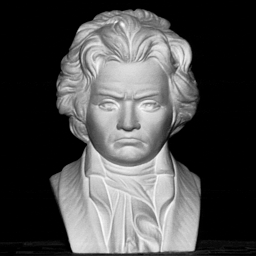
\includegraphics[width=0.2\textwidth]{DataCode2/Beethoven} &
    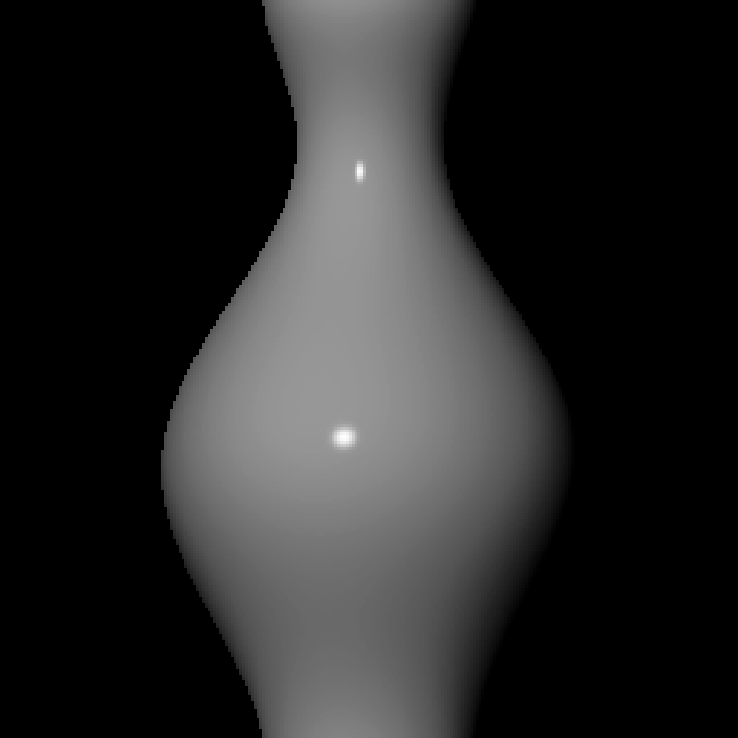
\includegraphics[width=0.2\textwidth]{DataCode2/shiny_vase}& 
    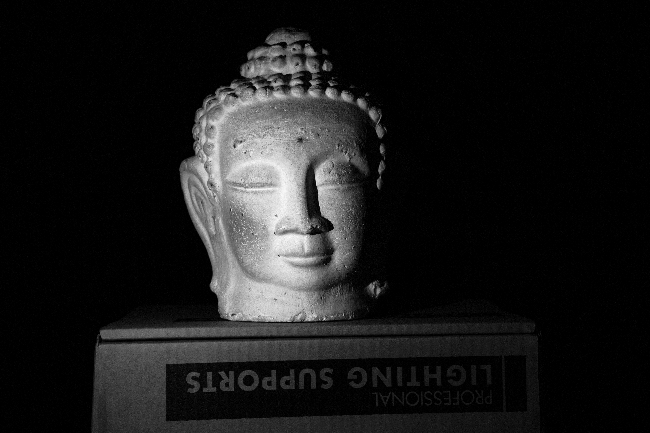
\includegraphics[width=0.2\textwidth]{DataCode2/Buddha3} &
    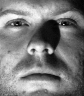
\includegraphics[width=0.2\textwidth]{DataCode2/face12}    
  \end{tabular}
  \caption{A few images out of the different datasets}
\end{figure}

For both all datasets
manipulation and reshaping is very important to maintain good
performances.  Both Matlab and Python/Numpy allow you to extract a
subarray as a list of value, and affects a list of value to an image
subarray. Woodham's estimation can be vectorised.  
You may want to look at integration source code to see how Python allows for 
these type of manipulations.

When using RANSAC, however, an estimation of albedo and normal will have to be performed
one pixel at a time.

\section{A bit of modelling}
You shoud provide brief answers to the following points. No need to elaborate too much.
\begin{itemize}
\item Write for a generic pixel, light source and normal, Lambert's law in its simplest form.
\item How is Lambert's law modified to deal with self shadows.
\item What about cast shadows? Comment
  on the difference between the two.
\item Comment on the modelling limits of Lambert's law.
\item How can we obtain an estimate of albedo and normals in Woodham's approach to
  Photometric Stereo. Write the equation.
\item What should be done if one uses RANSAC. Please describe. It will help you when
  implementing the RANSAC based estimation.
\end{itemize}




\section{Beethoven Dataset}

\texttt{Beethoven} is a synthetic and clean dataset, with exactly 3
images. If $nz$ is the number of pixels inside the non-zero part of
the mask, You should create an array $J$ of size/shape $(3,nz)$ and
obtain the albedo modulated normal field as $M=S^{-1}J$. With it,
extract the albedo within the mask, display it as a 2D image.  Then
extract the normal field by normalizing $M$, extract its components
$n1$, $n2$, $n3$. Solve for depth and display it at different view
points. 


\section{mat\_vase Dataset}

\texttt{mat\_vase} is a synthetic and clean dataset, with exactly 3
images. If $nz$ is the number of pixels inside the non-zero part of
the mask, You should create an array $J$ of size/shape $(3,nz)$ and
obtain the albedo modulated normal field as $M=S^{-1}J$. With it,
extract the albedo within the mask, display it as a 2D image.  Then
extract the normal field by normalizing $M$, extract its components
$n1$, $n2$, $n3$. Solve for depth and display it at different view
points. 

\section{shiny\_vase Dataset}

\texttt{shiny\_vase} is a synthetic and clean dataset, however not
respecting Lambert's law, which cannot cope with specularities.
It also consists of  exactly 3
images. If $nz$ is the number of pixels inside the non-zero part of
the mask, You should create an array $J$ of size/shape $(3,nz)$ and
obtain the albedo modulated normal field as $M=S^{-1}J$. With it,
extract the albedo within the mask, display it as a 2D image.  Then
extract the normal field by normalizing $M$, extract its components
$n1$, $n2$, $n3$. Solve for depth and display it at different view
points. Comment on what happens here.

Do you think that RANSAC could provide a better estimation of normals? Explain.  You
should try and replace Woodham's first step (via inverse/pseudoinverse) with RANSAC
estimation. The \texttt{threshold} parameter in \texttt{ransac\_3dvector()} should no more
than be 2.0. After the estimation for each pixel, extract the normals and the
albedo. Display and comment on the results. Do they differ from Woodham's estimation?  Try
then to make the estimated normal field smoother using the
\texttt{smooth\_normal\_field()} function. You may experiment with the \texttt{iters}
parameter.



\section{Buddha Dataset}

\texttt{Buddha} is real dataset, with exactly 10
images. If $nz$ is the number of pixels inside the non-zero part of
the mask, You should create an array $J$ of size/shape $(10,nz)$ and
obtain the albedo modulated normal field as $M=S^\dagger J$ (the pseudo-inverse). With it,
extract the albedo within the mask, display it as a 2D image.  Then
extract the normal field by normalizing $M$, extract its components
$n1$, $n2$, $n3$. Solve for depth and display it at different view
points.

You should try and replace Woodham's first step (via inverse/pseudoinverse) with an
estimation using RANSAC. The \texttt{threshold} parameter in \texttt{ransac\_3dvector()}
should be \textbf{at least} 25.0 Experiment with it.  After the estimation for each pixel,
extract the normals and the albedo. Display and comment on the results.  Try then to make
the estimated normal field smoother using the \texttt{smooth\_normal\_field()}
function. You may experiment with the \texttt{iters} parameter.


\section{face Dataset}
\texttt{Buddha} is real dataset, with exactly 27 images. If $nz$ is the number of pixels
inside the non-zero part of the mask, You should create an array $J$ of size/shape
$(27,nz)$ and obtain the albedo modulated normal field via RANSAC with a threshold of 10.0
Try then to make the estimated normal field smoother using the
\texttt{smooth\_normal\_field()} function. You may experiment with the \texttt{iters}
parameter. Report your results.



\end{document}
